\chapter{Wstęp}
\label{cha:introduction}
Założeniem projektu, było stworzenie modułu sensora, zgodnego ze standardem mikroBUS\texttrademark. Zespół, korzystając z okazji na zdobycie nowych umiejętności, zdecydował się rozszerzyć założenia projektowe o dwa dodatkowe sensory (co daje łącznie trzy układy pomiarowe na jednej płytce). Układy te, komunikują się z mikroprocesorem STM32F103 znajdującym się na tej samej płyce. W procesorze, dane są przetwarzane, nakładając dodatkową warstwę abstrakcji dla obsługi sensorów. Z płytką, można komunikować się przy użyciu interfejsu UART. Dodatkowym założeniem projektu, było różne podejście do tworzenia oprogramowania, każdego z członków zespołu. Zdecydowano, że jeden będzie tworzyć kod, testując go z mikroprocesorem STM32F4, kolejny bezpośrednio na wykonanej płyce, a ostatni, bez bezpośredniej styczności ze sprzętem. Podejście to, pozwoliło spojrzeć na pojekt z innej perspektywy, jak gdyby zespół był większy i rozproszony. Całe proces tworzenia był kontrolowany przy użyciu platformy Github, pozwalającej na wygodną kontrolę wersji oraz dyskusję nad kolejnymi zmianami w kodzie. \newline
W niniejszym sprawozdaniu, skupiono się przede wszystkim na procesie tworzenia modułu oraz popełnionych błędach, nie pomijając krótkiego wstępu teoretycznego. Całość, zakończona jest wnioskami na temat procesu oraz zdobytych umiejętności.
\section{mikroBUS\texttrademark}
MikroBus\texttrademark jest standardem definiującym układ gniazd oraz wyprowadzeń na płytce, zawierającej układ scalony (np. sensor). Standard opisuje również dokładne wymiary płytki, a także narzuca warstwę nadruków na płytce. Założeniem mikroBUS\texttrademark, jest umożliwienie szybkiego i łatwego rozbudowywania układów na rzecz prototypowania. Dostarczane przez wielu producentów płytki z gotowymi gniazdami, pozwalają w prosty sposób uruchomić dowolny sensor, a następnie stworzyć dla niego oprogramowanie. Tym samym, mikroBUS\texttrademark okazuje się świetną alternatywą dla niestabilnych płytek stykowych. Na rysunku \ref{img:mikrobus_pinout} przedstawiono zdefiniowany w standardzie pinout. \newline
Ze względu na zmienione założenia projektu, stworzona płytka zgadza się ze standardem co do wyprowadzeń i wymiarów, jednak nie posiada naniesionych nadruków. Wynika to wprost z braku miejsca, na płytce. Dodatkowo, kilka sensorów na jednej płytce, również nie jest zgodne ze standardem.

\begin{figure}[H]
    \centering
    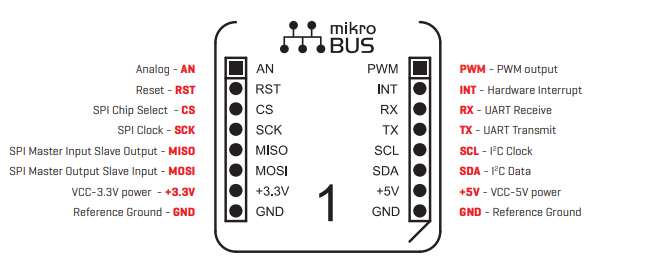
\includegraphics[width=12cm]{Graphics/mikrobus_pinout.png}
    \caption{Specyfikacja wyprowadzeń mikroBUS\texttrademark \cite{mikrobus_specification}}
    \label{img:mikrobus_pinout}
\end{figure}


\section{STM32F103}
Do stworzenia projektu, wybrano procesor STM32F103C8 z rdzeniem ARM\textregistered Cortex\textregistered-M3. Wybór, podyktowany był przede wszystkim dostępnością, ponieważ układ ten, w obudowach LQFP48 znajdował się w prywatnych zasobach zespołu. Obecnie, na rynku dostępne jest niewiele procesorów, a części elektroniczne są drogie. Z tego powodu, zdecydowano się korzystać z tego, co było dostępne. Nie oznacza to jednak, że procesor ten był pod jakimkolwiek względem ograniczający. Najistotniejszymi z jego cech są:
\begin{itemize}
    \item 2 interfejsy I$^2$C
    \item 3 interfejsy USART
    \item 2 interfejsy SPI
    \item Zasilanie 2.0 - 3.6V
    \item Zewnętrzny zegar 4 - 16MHz
    \item 12-bitowe, wielokanałowe przetworniki A/D
\end{itemize}
Układ, programowany jest przy użyciu interfejsu SWD oraz programatora ST-link. Fakt ten, znacząco ułatwił wykonanie działającego układu. Ze względu na przyjęte założenia i wybrane sensory, wybrany procesor bardzo dobrze wpasowywał się w projekt. Dla wykonania oprogramowania, istotne były również dostarczone przez ST biblioteki oraz oprogramowanie STM32CubeMX, wprowadzające wysoki poziom abstrakcji w tworzeniu oprogramowania. Pozwoliło to uniknąć często czasochłonnego, ręcznego pisania do rejestrów procesora, w celu konfiguracji peryferiów. Były również momenty, w których HAL okazał się problemem, co wspomniane zostało w dalszej części sprawozdania.

\section{STS30}

Sensor STS30-DIS marki Sensirion to cyfrowy, precyzyjny sensor temperatury. Wybraliśmy go jako przykładowy sensor działający po I$^2$C, oraz będący bardzo dobrze udokumentowany przez producenta. Oferuje dokładność 0.2 ℃ w zakresie temperatur 0-60 ℃, oraz funkcje takie jak wbudowane ogrzewanie, rejestr statusu, zmienny adres, soft reset po I$^2$C i wiele innych. Wszystkie dane z sensora są weryfikowane CRC-8.

\section{BMP280}

Krótki opis sensora Matiego

\section{MQ2}

Krótki opis sensora Matiego

\section{Makefile}
Jak wspomniano we wstępie, jednym z założeń, było tworzenie oprogramowania równolegle, na dwóch różnych procesorach. STM32F1 i STM32F4. Procesory te, należąc do zupełnie różnych rodzin, korzystają z innych bibliotek, a do ich konfiguracji niejednokrotnie wymagane są różne kroki. Z tego powodu, w projekcie wykorzystano program \emph{Make}. Pozwala on, na podstawie pliku konfiguracyjnego \emph{makefile}, zdefiniować sposób kompilacji oraz ścieżki bibliotek wykorzystywanych przez kod. Narzędzie to, jest stosunkowo proste w konfiguracji, a jej przykłady są ogólnodostępne w internecie. Dodatkowym argumentem przemawiającym za jego wykorzystaniem, była chęć jego przetestowania w praktyce.

\section{Github}
Github, to serwis internetowy pozwalający przechowywać projekty z wykorzystaniem systemu kontroli wersji. Korzysta on z systemu Git opublikowanego na licencji GNU GPL 2 (wolne i otwarte oprogramowanie). System ten, jest obecnie wykorzystywany przez wielu programistów, a jego znajomość często wymagana jest przez pracodawców. Github, poza kontrolą wersji, dostarcza wygodne i przejrzyste środowisko w przeglądarce, pozwalające programistom na np. przegląd kodu współpracowników. Fakt ten, został wykorzystany podczas tworzenia projektu. Pozwoliło to nie tylko na poprawienie jakości tworzonego oprogramowania, ale również skonfrontowanie różnych podejść do współpracy nad kodem.
